%%%%%%   TIPO DE DOCUMENTO: Artículo   %%%%%%
\documentclass[letterpaper,11pt,twoside]{report}

\usepackage[spanish]{babel} %Idioma
\usepackage{graphicx} %Imágenes
\usepackage[utf8]{inputenc} %Acentos
\usepackage{hyperref} %Links
\usepackage{xspace}

\usepackage{listings}
\usepackage{verbatim}
\usepackage{amsmath, amssymb}
\usepackage{amsmath}
\usepackage[active]{srcltx}
\usepackage{amssymb}
\usepackage{amscd}
\usepackage{makeidx}
\usepackage{amsthm}
\usepackage{algpseudocode}
\usepackage{algorithm}
\renewcommand{\baselinestretch}{1}
\setcounter{page}{1}
\setlength{\textheight}{21.6cm}
\setlength{\textwidth}{14cm}
\setlength{\oddsidemargin}{1cm}
\setlength{\evensidemargin}{1cm}
\pagestyle{myheadings}
\thispagestyle{empty}
\markboth{\small{Tarea 2, Jorge Martinez.}}{\small{.}}
\date{}

\begin{document}
	\centerline{\bf Redes de computadoras, \today}
	\centerline{}
	\begin{center}
		\Large{\textsc{Transferencia confiable, TCP y control de congesti\'on}}
	\end{center}
	
	\centerline{}
	\centerline{\textbf{Martínez Buenrostro Jorge Rafael}}
	\centerline{}
	
	\centerline{$correo, molap96@gmail.com$}
	
        \centerline{Universidad Aut\'onoma Metropolitana} 
	\centerline{Unidad Iztapalapa, M\'exico}
	
    \section*{Knowledge Checks}

\subsection*{Connectionless Transport: UDP}
    \subsubsection*{UDP header files}
    \begin{itemize}
        \item Which fields are in a UDP segment header?
        \item[] Source port, destination port, length (of UDP header plus payload),
        internet 
        \item Why is the UDP header length field needed?
        \item[] Because the payload section can be of variable length, and this lets UDP know where the
        segment ends
        \item Over what set of bytes is the checksum field in the UDP header computed over?
        \item[] The entire UDP segment, except the checksum field itself, and the IP senders and receive
        address fields
        \item The next statements are true about a checksum:
        \begin{itemize}
            \item A checksum is computed at a sender by considering each byte within a packet
            as a number, and then adding these numbers (each number representing a bytes)
            together to compute a sum (which is known as a checksum)
            \item The sender-computed checksum value is often included in a checksum field
            within a packet header
            \item The receiver of a packet with a checksum field will add up the received
            bytes, just as the sender did, and compare this locally-computed checksum with the
            checksum value in the packet header. If these two values are \textbf{different}
            then the receiver \textbf{knows} that one of the bits in the received packet has been changed
            during transmission from sender to receiver.
        \end{itemize}
        \item Compute the Internet checksum for these two 16-bit words: 11110101 11010011 and 10110011 01000100
        \item[] To compute the Internet checksum of a set of 16-bit words, we compute the one's complement sum 
        of the two words. That is, we add the two numbers together, making sure that any carry into the 17th bit
        of this initial sum is added back into the 1's place of the resulting sum); we then take the one's
        complement of the result. This means that the Internet checksum is \textbf{01010110 11100111}
        \item Compute the Internet checksum for these two 16-bit words: 01000001 11000100 and 00100000 00101011
        \item[] To compute the Internet checksum of a set of 16-bit words, we compute the one's complement sum 
        of the two words. That is, we add the two numbers together, making sure that any carry into the 17th bit
        of this initial sum is added back into the 1's place of the resulting sum); we then take the one's
        complement of the result. This means that the Internet checksum is \textbf{10011110 00010000}
        \item[NOTE] https://traductordebinario.com/calculadora-de-sumas-binario/ 
        \item[NOTE] https://www.allmath.com/es/calculadora-del-complemento-a-uno.php
        \item When computing the Internet checksum for two numbers, a single flipped bit (i.e., in just one of
        the two numbers) will always result in a changed checksum
        \item When computing the Internet checksum for two numbers, a single flipped bit (i.e., in just one of
        the two numbers) will NOT result in a changed checksum.
        \item Now consider the UDP datagram (and the IP datagram that will encapsulate it) sent in reply by the
        application on host 128.119.40.186  to the original sender host, labeled B in the figure above.
        \begin{figure}[H]
            \centering
            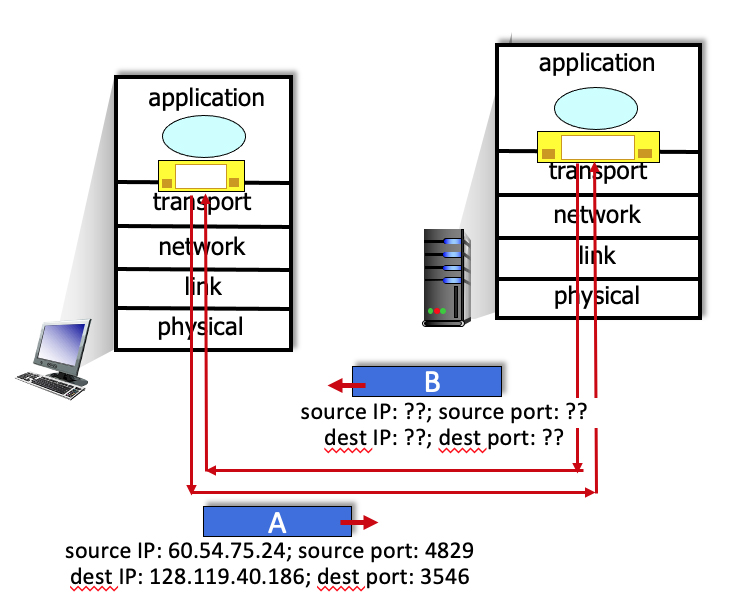
\includegraphics[width=0.5\textwidth]{img/3.3.9.jpg}
            \label{fig:UDP}
        \end{figure}
        \begin{itemize}
            \item The source port number of the UDP segment (B) sent in reply is: \textbf{3546}
            \item The source IP address of the IP datagram containing the UDP segment (B) sent in reply is: \textbf{128.119.40.186}
            \item The destination port number of the UDP segment (B) sent in reply  is: \textbf{4829}
            \item The destination IP address of the IP datagram containing the UDP segment (B) sent in reply is: \textbf{60.54.75.24}
        \end{itemize}
    \end{itemize}

    \subsubsection*{UDP segment length field}
    \begin{itemize}
        \item Why is the UDP header length field needed?
        \item[] Because the payload section can be of variable length, and this lets UDP know where the segment ends
        \item Over what set of bytes is the checksum field in the UDP header computed over?
        \item[] The enire UDP segment, except the checksum field itself, and the IP sender and recieve address fields
        \item The next statements are true about a checksum:
        \begin{itemize}
            \item A checksum is computed at a sender by considering each byte within a packet as a number, and then
            adding these numbers (each number representing a bytes) together to compute a sum
            \item The sender-computed checksum value is often included in a checksum field within a packet header
            \item The receiver of a packet with a checksum field will add up the received bytes, just as the sender did,
            and compare this locally-computed checksum with the checksum value in the packet header. If these two
            values are \textbf{different} then the receiver \textbf{knows} that one of the bits in the received packet
            has been changed during transmission from sender to receiver
        \end{itemize}
        \item Compute the Internet checksum for these two 16-bit words: 11110101 11010011 and 10110011 01000100
        \item[] To compute the Internet checksum of a set of 16-bit words, we compute the one's complement sum 
        of the two words. That is, we add the two numbers together, making sure that any carry into the 17th bit
        of this initial sum is added back into the 1's place of the resulting sum); we then take the one's
        complement of the result. This means that the Internet checksum is \textbf{01010110 11100111}
        \item Compute the Internet checksum for these two 16-bit words: 01000001 11000100 and 00100000 00101011
        \item[] To compute the Internet checksum of a set of 16-bit words, we compute the one's complement sum 
        of the two words. That is, we add the two numbers together, making sure that any carry into the 17th bit
        of this initial sum is added back into the 1's place of the resulting sum); we then take the one's
        complement of the result. This means that the Internet checksum is \textbf{10011110 00010000}
        \item When computing the Internet checksum for two numbers, a single flipped bit will always result in a 
        changed checksum
        \item When computing the Internet checksum for two numbers, a single flipped bit in each of the two numbers
        will NOT result in a changed checksum
    \end{itemize}

    \subsubsection*{Internet Checksum and UDP}
    \begin{itemize}
        \item 
    \end{itemize}

    \subsubsection*{What is checksum?}
    \subsubsection*{Computing the internet Checksum (1)}
    \subsubsection*{Computing the internet Checksum (2)}
    \subsubsection*{UDP Checksum: how good is it?}
    \subsubsection*{UDP Checksum: how good is it?}
    \subsubsection*{IP addresses and port numbers in a UDP segment sent in reply}

\subsection*{Principles of Reliable Data Transfer}
    \subsubsection*{Reliable data transfer protocol mechanisms}
    \subsubsection*{Cumulative ACK}
    \subsubsection*{Stop-and-wait: channel utilization}
    \subsubsection*{Channel utilization with pipelining}
    \subsubsection*{Channel utilization with pipelining (more)}
    \subsubsection*{Pipelining}
    \subsubsection*{Packet buffering in Go-Back-N}
    \subsubsection*{Packet buffering in Go-Back-N (more)}
    \subsubsection*{Receiver operation in Selective Repeat}
    \subsubsection*{Receiver operation in Selective Repeat (more)}


\subsection*{Connection-oriented Transport: TCP}
    \subsubsection*{Reliable data transfer protocol mechanisms}
    \subsubsection*{Cumulative ACK}
    \subsubsection*{Stop-and-wait: channel utilization}
    \subsubsection*{Channel utilization with pipelining}
    \subsubsection*{Channel utilization with pipelining (more)}
    \subsubsection*{Pipelining}
    \subsubsection*{Packet buffering in Go-Back-N}
    \subsubsection*{Packet buffering in Go-Back-N (more)}
    \subsubsection*{Receiver operation in Selective Repeat}
    \subsubsection*{Receiver operation in Selective Repeat (more)}

\subsection*{Principles of Congestion Control}
    \subsubsection*{Congestion control versus flow control}
    \subsubsection*{Two congested senders}
    \subsubsection*{Different approaches towards congestion control}

\subsection*{TCP Congestion Control}
    \subsubsection*{TCPs AIMD algorithm}
    \subsubsection*{TCPs AIMD algorithm (2)}
    \subsubsection*{TCPs Slowstart algorithm}
    \section*{Encaminamiento por vector-distancia, direccionamiento IP y detecci\'on de errores con CRC}

\begin{enumerate}
    \item Aplique el algoritmo de encaminamiento de vector-distancia a la siguiente topolog\'ia de red.
    \begin{enumerate}
        \item Indique el estado de las tablas de ruteo para las etapas de cold-start y luego para el env\'io de los primeros dos mensajes.
        \begin{table}[H]
            \begin{tabular}{@{}clcll@{}}
            \toprule
            From A to            & \multicolumn{1}{c}{Link} & Cost                 \\ \midrule
            A                    & local                    & 0                    \\ \bottomrule
            \end{tabular}
            \hfill
            \begin{tabular}{@{}clcll@{}}
                \toprule
                From B to            & \multicolumn{1}{c}{Link} & Cost                 \\ \midrule
                B                    & local                    & 0                    \\ \bottomrule
            \end{tabular}
            \hfill
            \begin{tabular}{@{}clcll@{}}
                \toprule
                From C to            & \multicolumn{1}{c}{Link} & Cost                 \\ \midrule
                C                    & local                    & 0                    \\ \bottomrule
            \end{tabular}
            \vfill
            \begin{tabular}{@{}clcll@{}}
                \toprule
                From D to            & \multicolumn{1}{c}{Link} & Cost                 \\ \midrule
                D                    & local                    & 0                    \\ \bottomrule
            \end{tabular}
            \hfill
            \begin{tabular}{@{}clcll@{}}
                \toprule
                From E to            & \multicolumn{1}{c}{Link} & Cost                 \\ \midrule
                E                    & local                    & 0                    \\ \bottomrule
            \end{tabular}
            \hfill
            \begin{tabular}{@{}clcll@{}}
                \toprule
                From F to            & \multicolumn{1}{c}{Link} & Cost                 \\ \midrule
                F                    & local                    & 0                    \\ \bottomrule
            \end{tabular}
            \vfill
        \end{table}


        \item Luego, indique el estado de las tablas de ruteo para el estado estacionario.
        \item Una vez alcanzado el estado estacionario , el enlace 6 se rompe. Descria la manera en c\'omo procede el protocolo hasta retomar
        un nuevo estado estacionario.
        \item ¿Qu\'e fen\'omeno podr\'ia causar un bucle de ruteo?
        \item Finalmente, ¿cu\'al protocolo en la pr\'actica implementa el algoritmo de vector-distancia? ¿cu\'al es la frecuencia de los mensajes
        de refresco y cu\'al es la finalidad de los mismos?

        \begin{figure}[H]
            \centering
            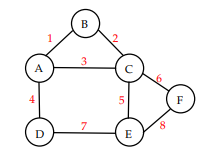
\includegraphics[width=0.35\textwidth]{img/Vector-distancia.png}
        \end{figure}
    \end{enumerate}

    \item Suponga que le han asignado el bloque de red 132.46.0.0/16 y que necesita configurar ocho subredes.
    \begin{enumerate}
        \item ¿Cu\'antos d\'igitos binarios se requieren para definir ocho subredes?
        \item Especifique el prefijo de red extendido que permite la creaci\'on de las 8 subredes.
        \item Exprese las direcciones de subred en formato binario y decimal.
        \item Enliste el rango de direcciones IP que pueden asignarse a la subred n\'umero 4.
        \item ¿Cu\'al es la direcci\'on de difusi\'on (\textit{broadcast}) de la subred n\'umero 4?
    \end{enumerate}

    \item Suponga que se le ha asignado el bloque de direcciones de red 200.30.1.0/24.
    \begin{enumerate}
        \item Defina un prefijo de red extendido que permita crear 20 estaciones en cada subred.
        \item ¿Cu\'al es el n\'umero m\'aximo de estaciones que pueden asignarse a cada subred?
        \item ¿Cu\'al es el n\'umero m\'aximo de subredes que pueden definirse?
        \item Especifique las subredes de 200.30.1.0/24 en formatos binario y decimal.
        \item Enliste las direcciones de estaci\'on que pueden asignarse a la subred 6.
        \item ¿Cu\'al es la direcci\'on de difusi\'on para la subred 2?
    \end{enumerate}

    \item Se le ha asignado a una organizaci\'on el n\'umero de red 140.20.0.0/16 y \'esta planea desarrollar VLSM. En el primer nivel de jerarqu\'ia,
    se necesitan configurar ocho subredes. La subred 1 necesita configurar 32 sub-redes y la subred 6 necesita configurar 16 sub-redes. Finalmente, la
    sub-red 6-14 necesita configurar 8 \(sub^2-subredes\).
    \begin{enumerate}
        \item Dibuje el \'arbil que ilustre la jerarqu\'ia necesaria para implementar VLSM.
        \item Especifique las ocho subredes 140.20.0.0/16.
        \item Enliste las direcciones de estaci\'on que pueden asignarse a la subred 3.
        \item Indique la direcci\'on de difusi\'on de la subred 3.
        \item Indique las 16 sub-redes de la subred 6.
        \item Enliste las direcciones de estaci\'on que pueden asignarse a la sub-subred 6-3.
        \item Indentifique la direcci\'on de broadcast para la sub-subred 6-3.
        \item Especifique las ocho \(sub^2-subredes\) de la sub-subred 6-14.
        \item Enliste las direcciones de estaci\'on que pueden asignarse en la \(sub^2-subred\) 6-14-2.
        \item Indentifique la direcci\'on de broadcast de la \(sub^2-subred\) 6-14-2.
    \end{enumerate}

    \item En el nivel de enlace de datos se utiliza frecuentemente el mecanismo de verificaci\'on de redundancia c\'iclica (\textit{CRC: Cyclic 
    Redundance Check}) para que una interfaz receptora concluya sobre si la trama recibida, \(T'\) contiene o no errores. Suponga que el mensaje
    a transmitir es \(M=1101011011\) y que el generador es \(G=10011\).
    \begin{enumerate}
        \item Encuentre la trama, \(T\) que env\'ia el transmisor.
        \item Realice la operaci\'on que ejecuta la interfaz receptora si el patr\'on de error inducido en el canal \(e=00000000000000\), ¿cu\'al 
        es la conclusi\'on del receptor?
        \item Realice lo mismo que en (b), pero ahora con un error inducido en el canal f\'isico \(e=00100000010011\), ¿cu\'al es la conclusi\'on
        del receptor?
        \item ¿Existe la posibilidad de que habiendo errores en \(T'\), la trama recibida, el receptor sea incapaz de detectarlos? Explique.
        \item Finalmente, realice (a)-(c) operando polinimialmente.
    \end{enumerate}
\end{enumerate}
\end{document}